\section{Motivation and Related Works}
\label{sec:snic:motivation}

\subsection{Benefits of Network Disaggregation}
\label{sec:snic:benefits}
As discussed in \S\ref{sec:snic:intro}, disaggregating network functionalities into a separate pool has several key benefits for data centers, some of which are especially acute for future disaggregated, heterogeneous data centers~\cite{LegoOS,last-cpu-hotos, FratOS-eurosys}.

\bolditpara{Flexible management and low development cost.}
Modern data centers are deploying an increasing variety of network tasks to endpoints, usually in different forms (\eg, software running on a CPU, fixed-function tasks built as ASIC in a NIC, software and programmable hardware deployed in a SmartNIC). 
It requires significant efforts to build and deploy them to different network devices on regular servers and to different types of disaggregated hardware devices.
After deployment, configuring, monitoring, and managing them on all the endpoints is also hard.
%, even in a homogeneous cluster.
In contrast, developing, deploying, and managing network tasks in a disaggregated network pool with homogeneous devices is easy and flexible.

\bolditpara{Independent scaling.}
It is easy to increase/decrease network hardware resources in a disaggregated network pool by adding/removing network devices in the pool. Without disaggregation, changing network resources would involve changing endpoints (\eg, upgrading or adding NICs).

\bolditpara{Access to large network resources.}
With disaggregation, an endpoint can potentially use the entire network pool's resources, far beyond what a single NIC or server can offer.
This is especially useful when there are occasional huge traffic spikes or peak usages of many \nt{}s.
Without network disaggregation, the endpoint would need to install a large NIC/SmartNIC that is bloated with features and resources not commonly used~\cite{SmartNIC-nsdi18,Caulfield-2018}.

Beside the above benefits, a major benefit of network disaggregation is cost savings. A consolidated network pool only needs to collectively provision for the peak aggregated traffic and the maximum total \nt{}s used by the whole rack at any single time.
In contrast, today's non-disaggregated network systems require each endpoint to provision for its individual peak traffic and maximum \nt{}s.
To understand how significant this cost is in the real world, we analyze a set of traces from both traditional server-based production data centers and disaggregated clusters.

\bolditpara{Server-based data center traffic analysis.}
To understand network behavior in server-based data centers, we analyze two sets of traces: a Facebook trace that consists of Web, Cache, and Hadoop workloads~\cite{facebook-sigcomm15}, and an Alibaba trace that hosts latency-critical and batch jobs together~\cite{alibaba-trace}. 

We first perform a consolidation analysis where we calculate the sum of peaks in each individual endhost's traffic (sum of peak) and the peak of aggregated traffic within a rack and across the entire data center (peak of sum). 
These calculations model the cases of no disaggregation, disaggregation and consolidation at the rack level and at the data-center level.
Figure~\ref{fig-fb-alibaba} shows this result for the two data centers. 
For both of them, a rack-level consolidation consumes one magnitude fewer resources than no consolidation.

We then analyze the load spikes in these traces
by comparing different endhosts' spikes and analyzing whether they spike at similar or different times, which will imply how much chance there is for efficient consolidation.
Specifically, we count how much time in the entire 1-day trace $X$ number of endhosts spike together.
Figure~\ref{fig-spike-var} shows that 55\% of the time only one or two servers spike together, and only 14\% of the time four or more servers spike together.
This result shows that servers mostly spike at different times, confirming the large potential of consolidation benefits.

{
\begin{figure*}
\begin{minipage}{0.25\textwidth}
\begin{center}
\centerline{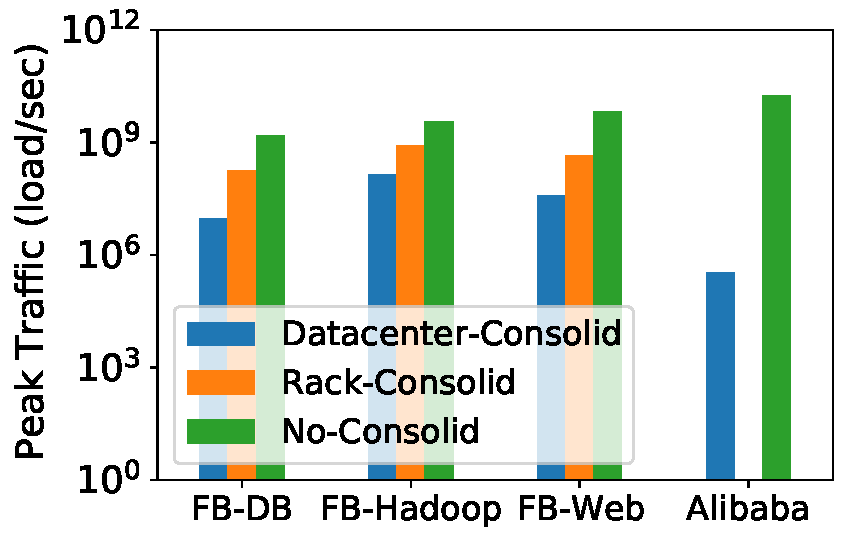
\includegraphics[width=\textwidth]{Figures/fig_fb_alibaba_trace.pdf}}
\vspace{-0.1in}
\mycaption{fig-fb-alibaba}{Consolidation Analysis of Facebook and Alibaba Traces.}
{
Load represent relative amount and have different units for FB and Alibaba.
}
\end{center}
\end{minipage}
\begin{minipage}{0.25\textwidth}
\begin{center}
\centerline{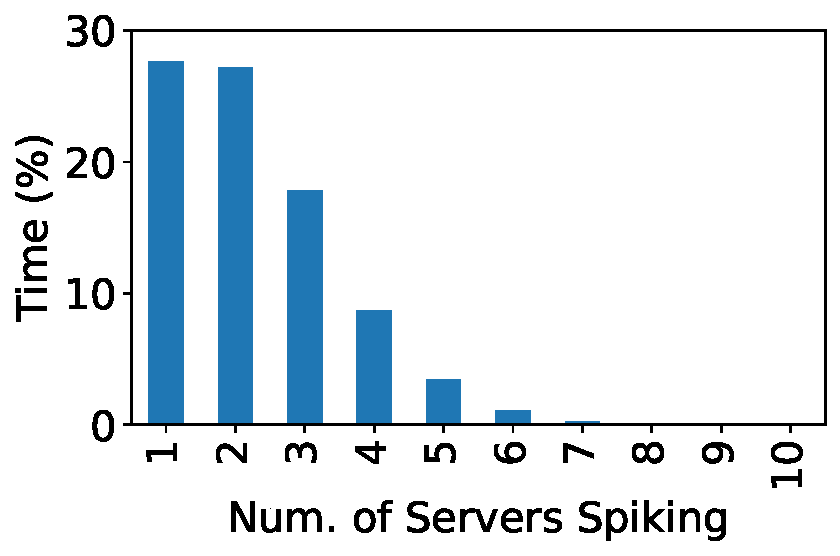
\includegraphics[width=\textwidth]{Figures/spike-trace-analysis.pdf}}
\vspace{-0.1in}
\mycaption{fig-spike-var}{Load Spike Variation across Endhosts in FB.}
{
}
\end{center}
\end{minipage}
\begin{minipage}{0.5\textwidth}
\begin{center}
\centerline{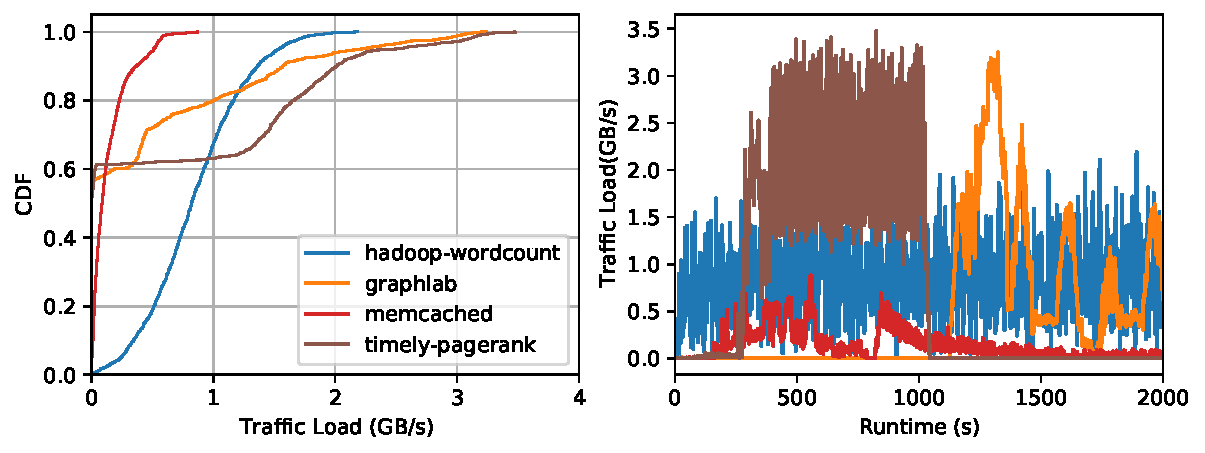
\includegraphics[width=\textwidth]{Figures/fig-osdi16-net-trace.pdf}}
\vspace{-0.15in}
\mycaption{fig-OSDI16NetTrace}{Network traffic for accessing disaggregated memory.}
{
}
\end{center}
\end{minipage}
\vspace{-0.15in}
\end{figure*}
}


\bolditpara{Disaggregated cluster traffic analysis.}
Resource disaggregation introduces new types of network traffic that used to be within a server, \eg, a CPU device accesses data in a remote memory device. 
If not handled properly, such traffic could add a huge burden to the data-center network~\cite{sirius-sigcomm20}.
To understand this type of traffic, we analyzed a set of disaggregated-memory network traces collected by Gao et al. using five endhosts~\cite{Gao16-OSDI}.
Figure~\ref{fig-OSDI16NetTrace} plots the CDF and the timeline of network traffic from four workloads.
These workloads all exhibit fluctuating loads, with some having clear patterns of high and low load periods.
We further perform a similar analysis using sum of peaks vs. peak of aggregated traffic as our server-based trace analysis.
Consolidating just five endhosts already results in 1.1\x\ to 2.4\x\ savings with these traces.


\subsection{Limitations of Alternative Solutions}
\label{sec:snic:related}

The above analysis makes a case for disaggregating and consolidating network tasks from individual servers and devices.
A question that follows is \textit{where} to host these \nt{}s and whether existing solutions could achieve the goals of network disaggregation and consolidation.

%
The first possibility is to host them at a \textbf{programmable ToR switch}. Programmable switches allow for configurable data planes, but they typically support only a small amount of computation at high line rates. SmartNICs, on the other hand, handle more stateful and complex computations but at lower rates. Transport protocol processing and encrypted communications are examples of complex network tasks better supported by a SmartNIC than a programmable switch. Moreover, existing programmable switches lack proper multi-tenancy and consolidation support~\cite{Wang-HotCloud20}. As a consequence, most data center designs require the use of SmartNICs even in the presence of programmable switches, and our proposal simply disaggregates SmartNIC-like capabilities into a consolidated tier.


Another possibility is upcoming \emph{multi-host SmartNICs} (e.g., Mellanox BlueField3) that are enhancements of today's \textbf{multi-host NICs}~\cite{ocp-nic,Intel-RedRockCanyon}. These NICs connect to multiple servers via PCIe connections and provide general-purpose programmable cores. Our work identifies three key extensions to such devices. (1) Our approach enables a greater degree of aggregation as we enable coordinated management of a distributed pool of network devices. (2) Moreover, in the case of these multi-host SmartNICs, \nt{}s that cannot be mapped to the NIC's fixed functions have to be offloaded as software. In contrast, \snic\ allows the acceleration of \nt{}s in hardware, enabling higher performance while tackling issues related to runtime reconfigurability of hardware. (3) Our approach provides adaptive mechanisms for adjusting to workloads and providing fair allocation of resources across applications. It is also worth noting that (1) and (3) can by themselves be used in conjunction with commercial multi-host SmartNICs to achieve a different software-based instantiation of our vision.

\textbf{Middleboxes} are a traditional way of running network functions inside the network either through hardware black-box devices that cannot be changed after deployment~\cite{aplomb-sigcomm20,comb-nsdi12,walfish-osdi04} or through server-based Network Function Virtualization (NFV) that enables flexible software-based middleboxes~\cite{clickos-nsdi14,e2-sosp15,metron-nsdi18,NFP-sigcomm17,parabox-sosr17}, but at the cost of lower performance~\cite{netbricks,netvm-nsdi14}.  Our deployment setting differs from traditional datacenter middleboxes: we target "nearby" disaggregation, as in the endhost or SmartNIC tasks are disaggregated to a nearby entity typically located on the same rack. Consequently, our mechanisms are co-designed to take advantage of this locality (e.g., we use simple hardware mechanisms for flow control between the end-host and the disaggregated networking unit). Further, we target network functionality that is expected either at the endhost itself or at the edge of the network, such as endhost transport protocols, applying network virtualization, enhancing security, which all require nearby disaggregation and are also not typically targeted by middleboxes. We do note that our dynamic resource allocation mechanisms are inspired by related NFV techniques, but we apply them in the context of reconfigurable hardware devices.

Finally, there are emerging \textbf{interconnections designed for disaggregated devices} such as Gen-Z~\cite{GenZ} and CXL~\cite{CXL}.
These solutions mainly target the coherence problem where the same data is cached at different disaggregated devices.
The transparent coherence these systems provide requires new hardware units at every device, in addition to a centralized manager.
\snic\ supports the disaggregation and consolidation of all types of network tasks and does not require specialized units at endpoints.
